In this section we compute geodesics in the hot phase studied in the previous section. We apply what we learned in chapters \ref{section 2} and \ref{section 3} about RT surfaces. We split our system into two separate systems (CFT$_1$ and CFT$_2$) and compute results as if we had two boundary CFTs with an end of the world brane at the wall\cite{chu2021page}.

\section{Ryu-Takayanagi surfaces in a single slice}

We start by considering a single slice. It consists of a CFT on a an interval of length $L$ bounded by two interfaces lying on the boundary of a BTZ geometry, fig. \ref{BCFT}. Joining the two slices together is a matter of the choice of the constant $c_j$ in eq. (\ref{mysolved}). Since the geodesics lengths are independent of this choice, separating these two slices won't affect the results. This is like the situation a BCFT \cite{chu2021page} but with 2 end of the world branes instead.

\begin{figure}
    \centering
    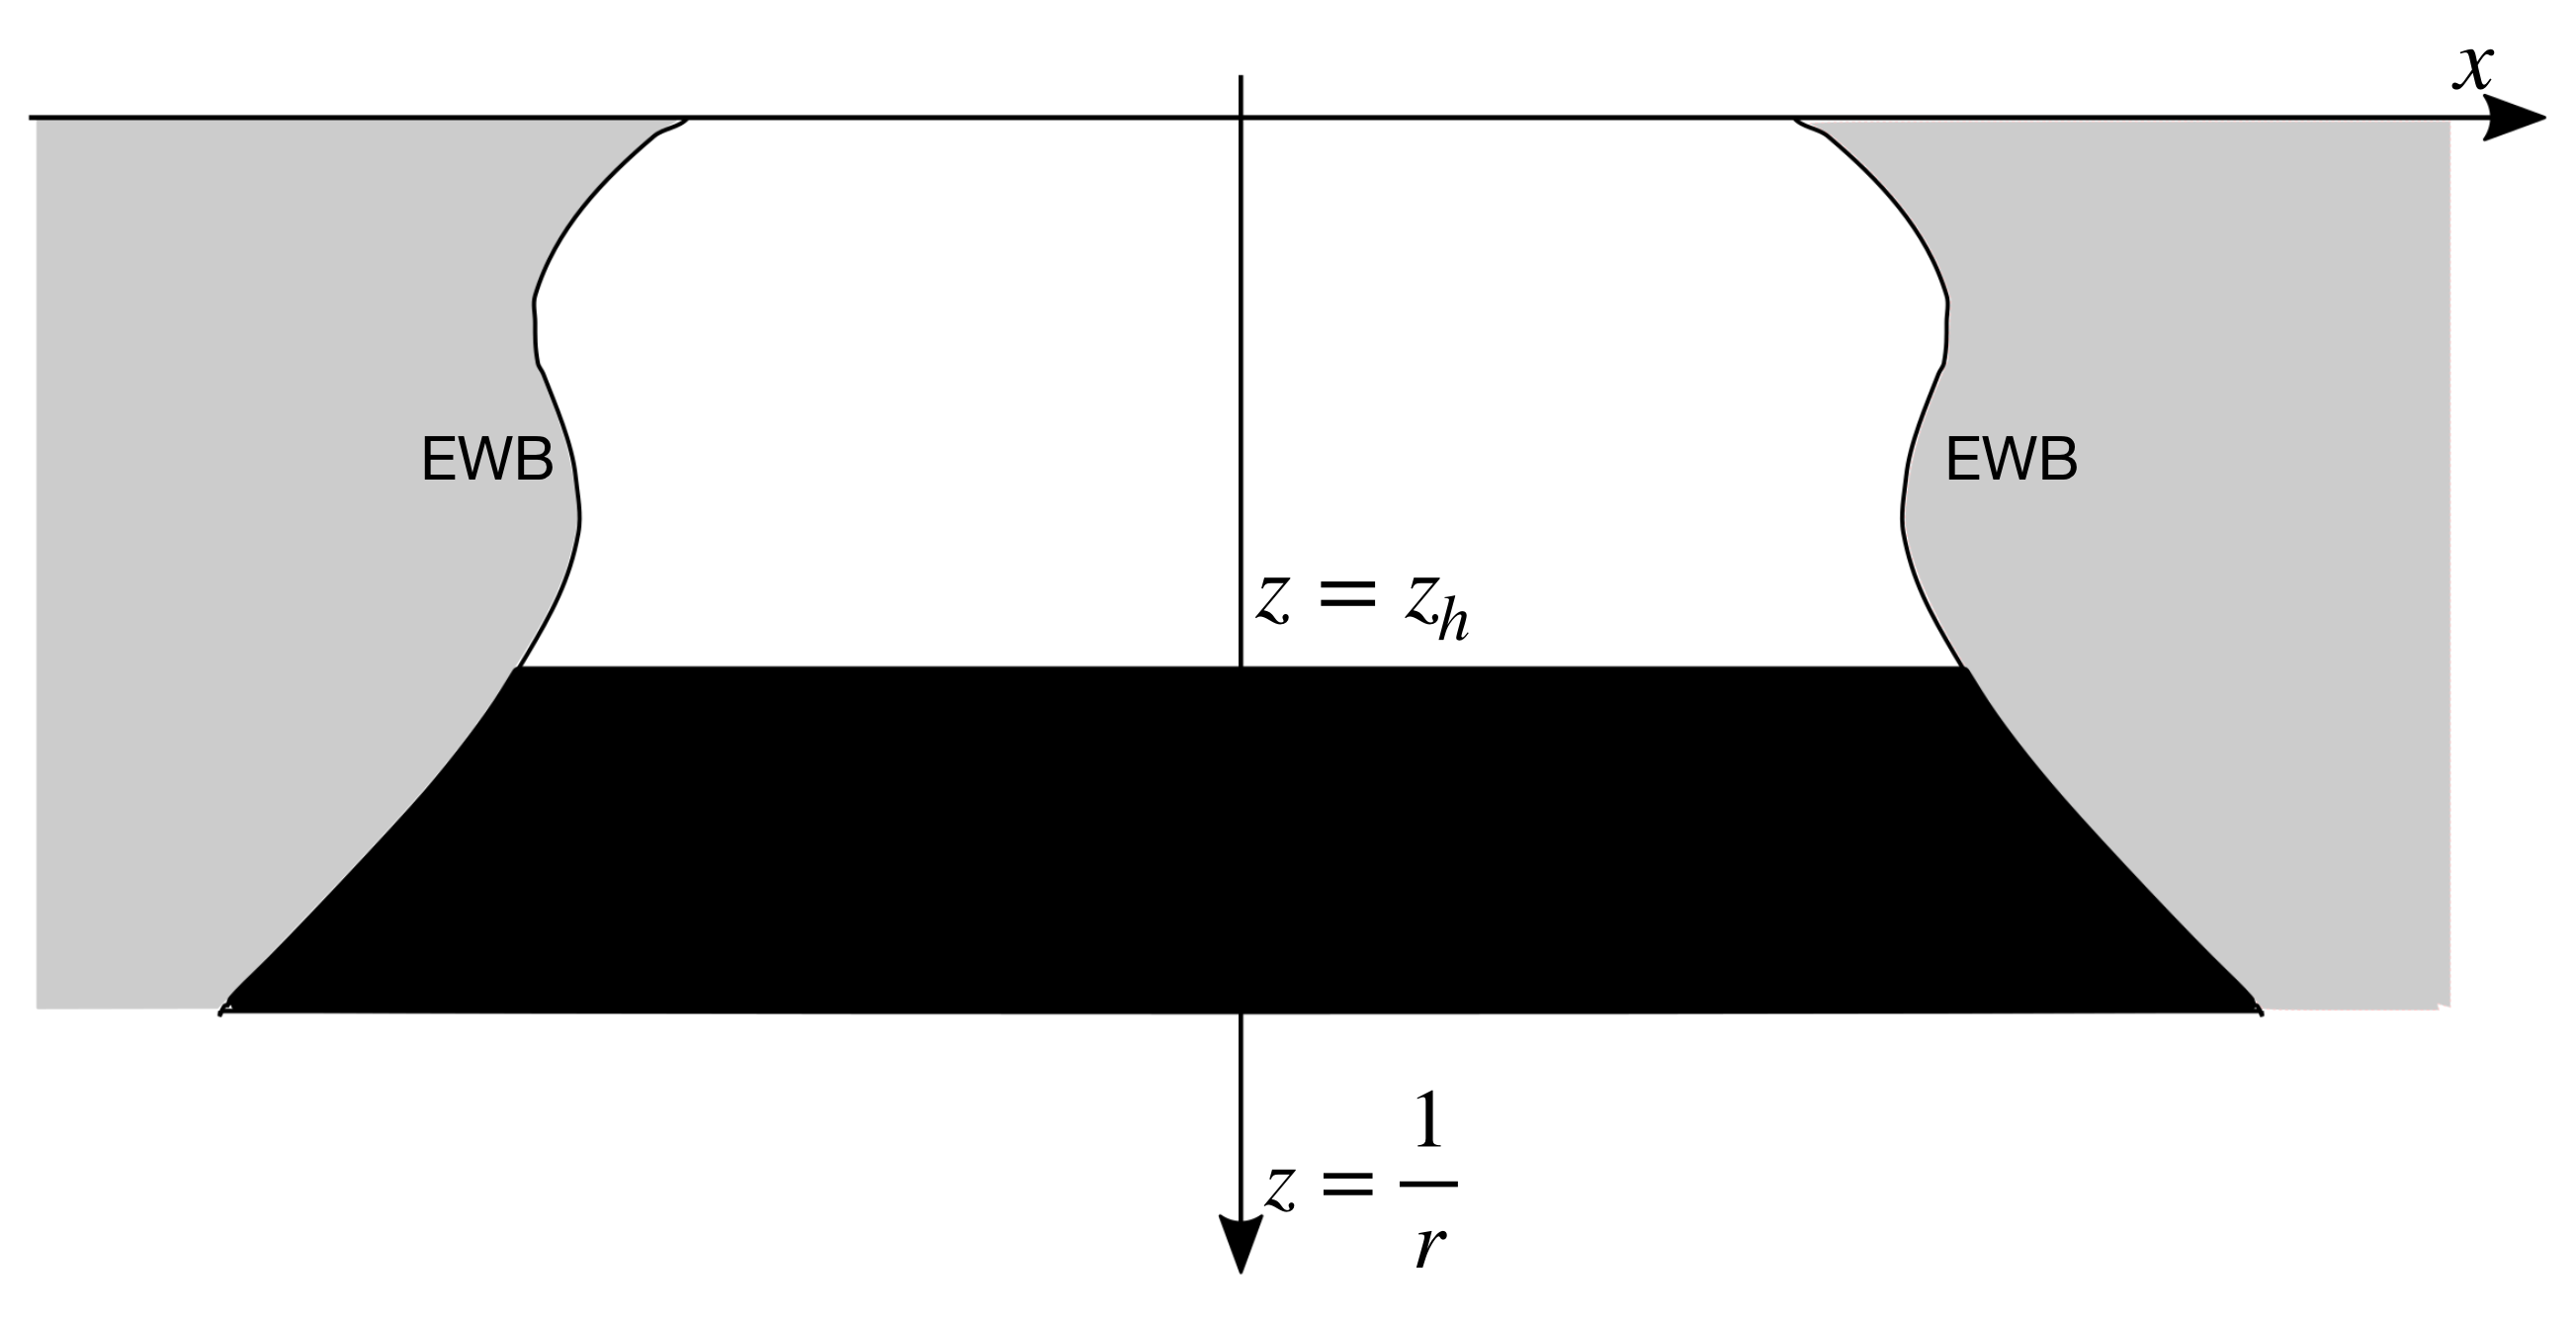
\includegraphics[width=0.9\textwidth]{figures/BCFT.png}
    \caption{BCFT with a BTZ geometry in the bulk. Since our original system features two walls, we represent here a BCFT with two end of the world branes. Here we used the (\ref{change of coord rz}) coordinates.}
    \label{BCFT}
\end{figure}

Computing RT surfaces goes back to computing space like geodesics. The geodesic equations in $(r,x)$\footnote{We don't write the slice index $j$ for clarity.} coordinates are
\begin{subequations}
    \label{geodesic equations}
    \begin{align}
        \ddot x &= -\frac{2\dot r\dot x}{r}\label{geodesic 1}\\
        \ddot r &= \frac{r\dot r}{r^2-M\ell^2} + \frac{r(r^2-M\ell^2)\dot x}{\ell^2},\label{geodesic 2}
    \end{align}
\end{subequations}
where the dot denotes a derivative with respect to the affine parameter $\lambda$.

The first equation (\ref{geodesic 1}) is just telling us that the tangential acceleration is vanishing and therefore the angular momentum is conserved,
\begin{equation}
    r^2\dot x=J.
\end{equation}

The second equation is more difficult to solve. We can treat this problem by considering the length of the geodesic between two endpoints $P_1$ and $P_2$,
\begin{equation}\label{Action}
    L = \ell\int d \phi\sqrt{\frac{r'^2}{r^2-M\ell^2}+r^2},
\end{equation}
where we made the following substitution $\phi=x/\ell$. The prime denotes a derivative with respect to $\phi$.

Treating $L$ as a one dimensional action, the energy conservation reads,
\begin{equation}
    \frac{r^2}{\sqrt{\frac{r'^2}{r^2-M\ell^2}+r^2}}= \frac{E}{\ell},
\end{equation}
where $E$ is a constant of integration. Rearranging this equation, we get,
\begin{equation}
    E^2r'^2 = \ell^2r^2(r^2-E^2)(r^2-r_h^2),
\end{equation}
where $r_h=\ell\sqrt{M}$. Integrating this equation a second time gives
\begin{equation}\label{solution phi}
    r(x) = \frac{E}{r_h}\frac{1}{\sqrt{\frac{E^2}{r_h^2\ell^2}\cosh^2\left(r_h\frac{x}{\ell}+c\right)-\sinh^2\left(r_h\frac{x}{\ell}+c\right)}}
\end{equation}
where $c$ is a constant of integration and can be set to 0 if we consider symmetric geodesics with respect to $x = 0$. Two geodesics are drawn in  fig. \ref{geodesic pic} between two infinite points separated by an arc of length $2x_0$ as well as two points on the wall. We impose different boundary conditions for each geodesic to find $E$.

Integrating (\ref{Action}) using (\ref{solution phi}), we find the length of the geodesic homologous to an interval of length $2x_0\ll L$ on the boundary,
\begin{equation}\label{S1}
    2\ell\ln\frac{2\sinh{\frac{r_h x_0}{\ell}}}{r_h \epsilon}.
\end{equation}
 
This is similar to what we find in eq. (\ref{length BTZ red}). The corresponding entanglement entropy is given by the RT formula,
\begin{equation}
    S = \frac{c}{3}\ln\frac{2\sinh{\frac{r_h x_0}{\ell}}}{r_h \epsilon}.
\end{equation}


\begin{figure}
    \centering
    \begin{subfigure}[b]{0.45\textwidth}
        \centering
        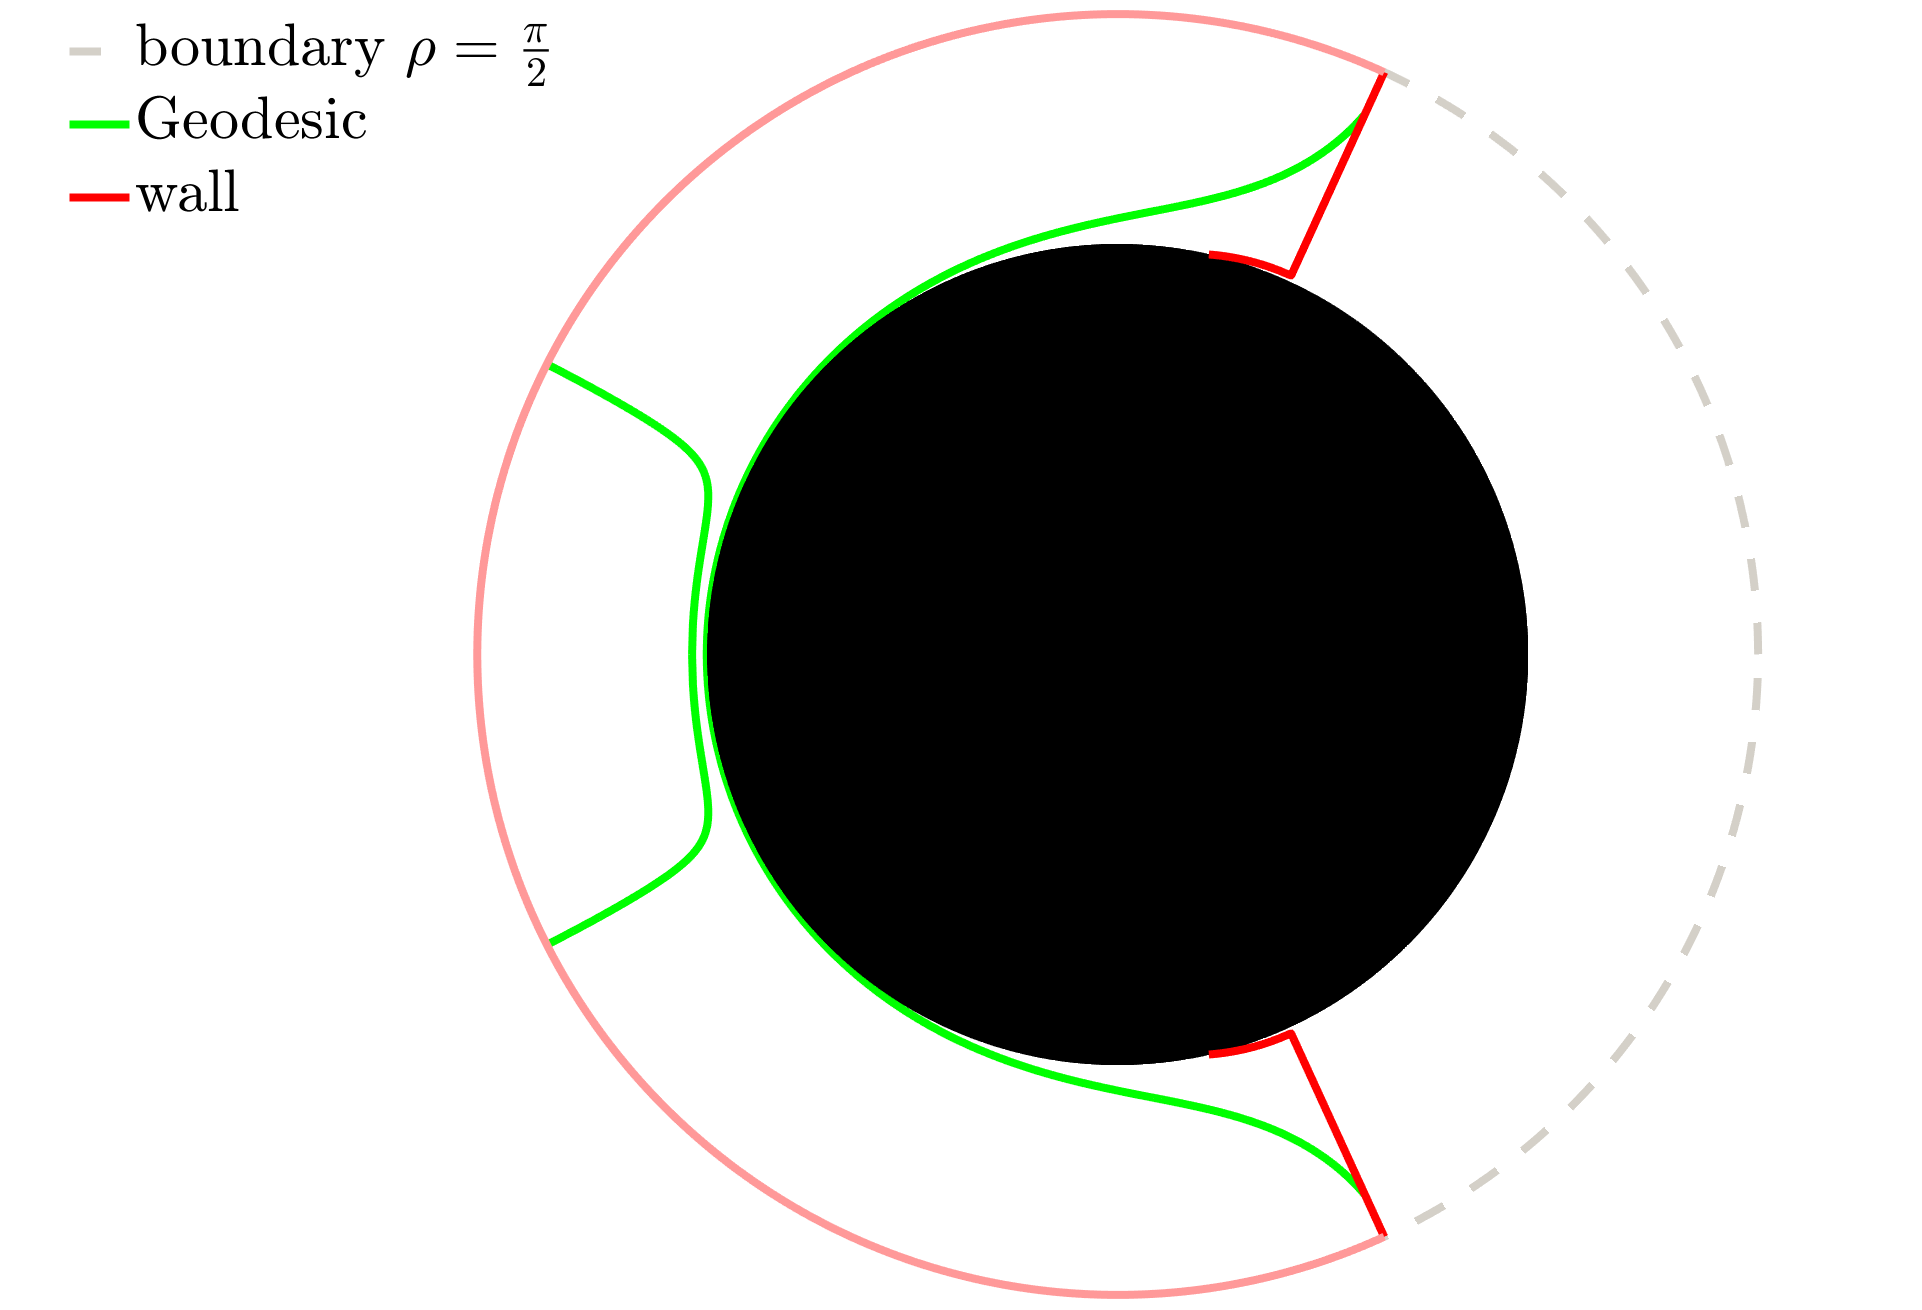
\includegraphics[width=\textwidth]{figures/geodesic_red.png}
        \label{greengeodesic}
    \end{subfigure}
    \hfill
    \begin{subfigure}[b]{0.45\textwidth}
        \centering
        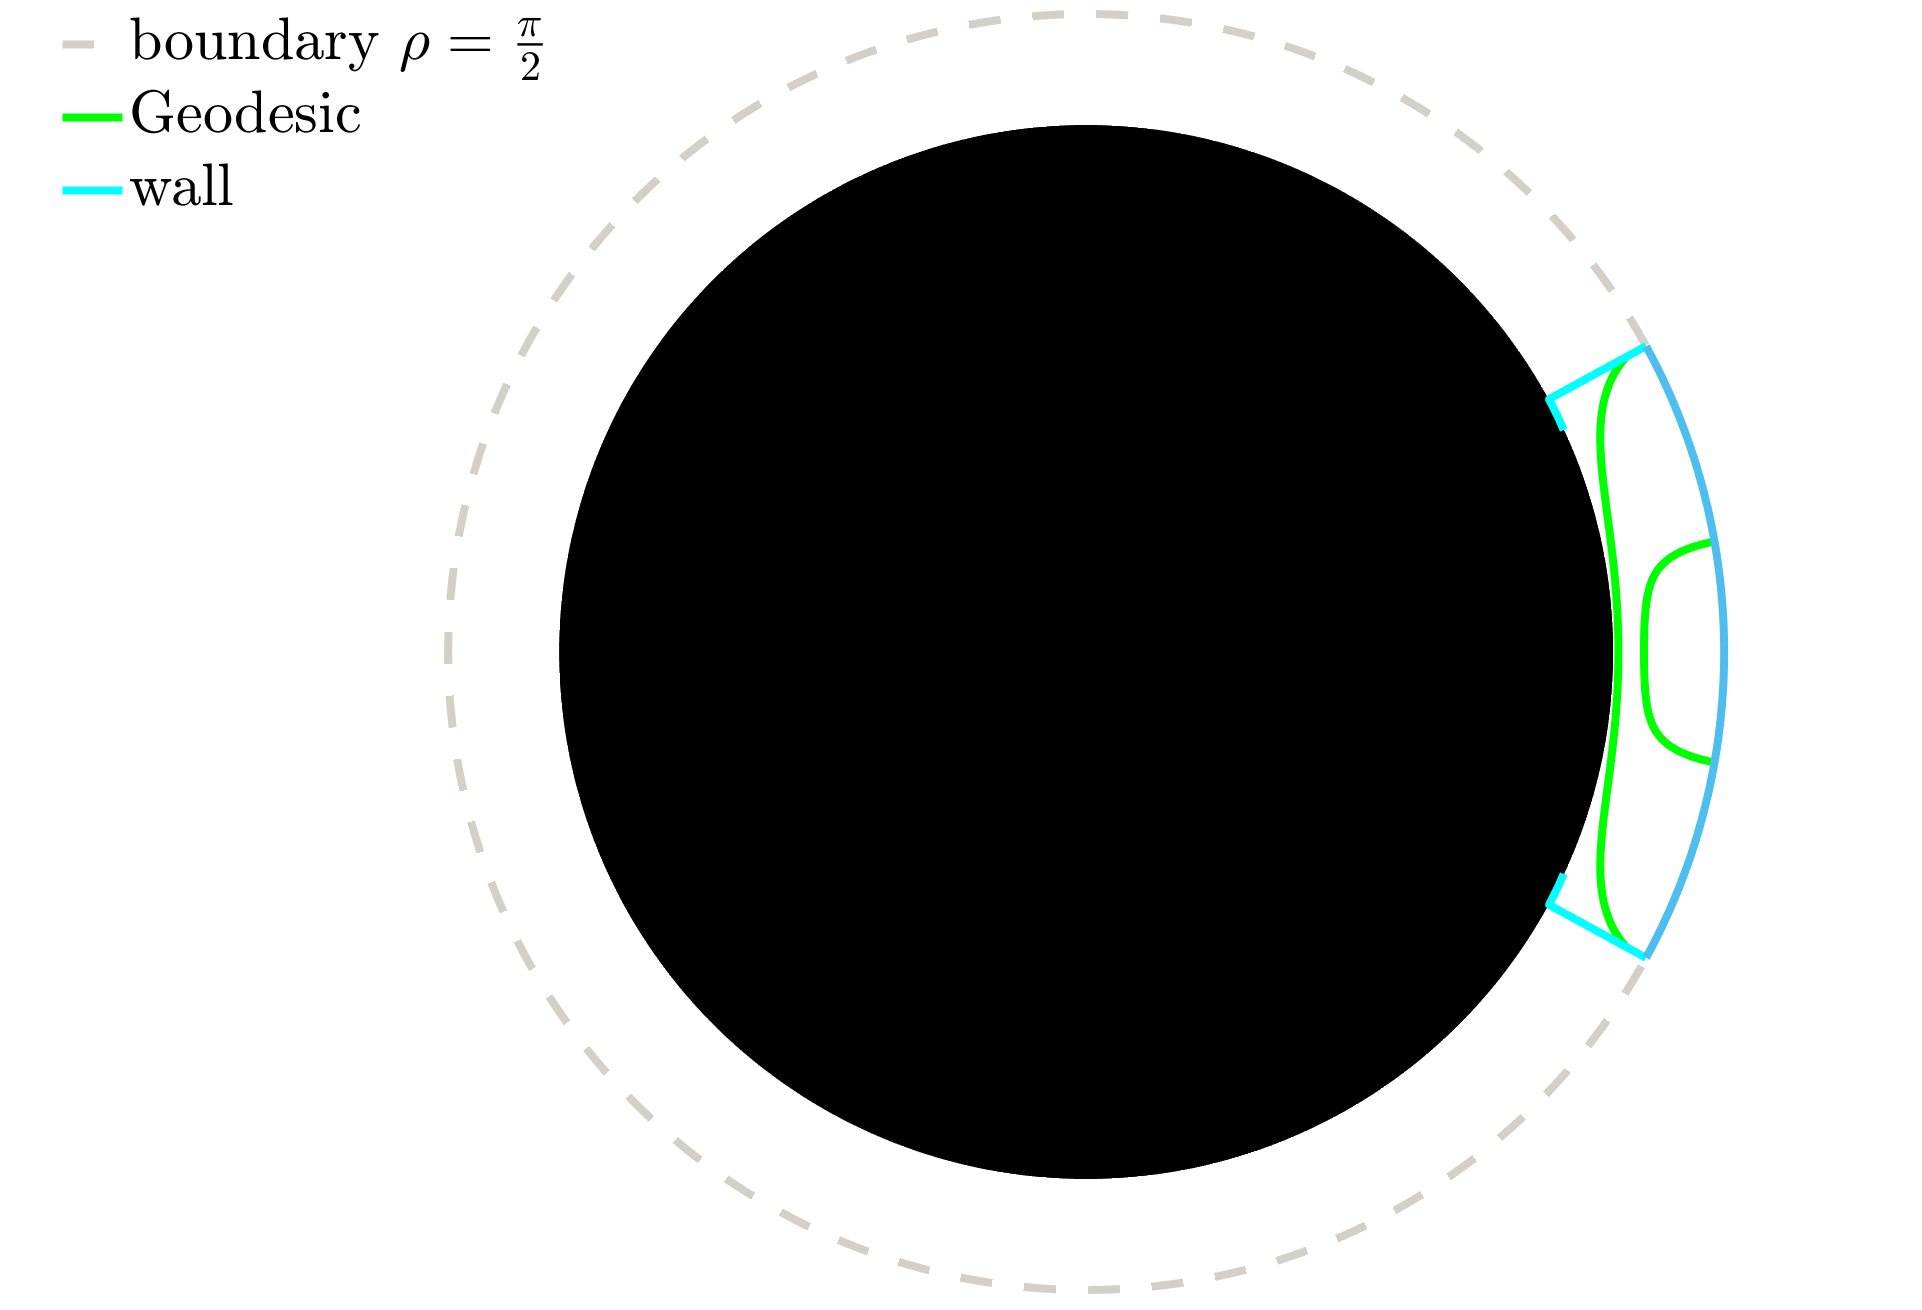
\includegraphics[width=\textwidth]{figures/geodesic_blue.png}
        \label{pinkgeodesic}
    \end{subfigure}
        \caption{Geodesics inside each slice between two symmetric points. One geodesic has its endpoints on the boundary, the other on the wall. For the red slice the geodesic with the the endpoints on the wall asymptotes the Horizon. We chose $\ell_1=0.1$ and $\ell_2=0.15$.}
        \label{geodesic pic}
\end{figure}

\section{Ryu-Takayanagi surfaces in the hot phase}

The system we are working on $[\text{H}2,\text{H}2]$ resembles a lot that of fig. \ref{fig_BTZ minimal surface}. In fact it is the same with the addition of a wall with different central charges on each side. Therefore, the computation of RT surfaces is somewhat similar to those in chapter \ref{section 3}, with the first possibility already computed in the previous section and the second one slightly different than eq. (\ref{second entropy}). 

More precisely, we compute the EE of the blue slice with a large number of degrees of freedom $c_2$ as was depicted in fig. \ref{QM 2}. The EE is that of an interval $A$ which includes all of $L_2$ and an finite part of $L_1$ of size $h$ of the same order as $L_2$. The RT surfaces correspond to geodesics linking two symmetric points on the red slice boundary. They can be of two kinds: either they stay in the same slice (the red one) or they cross the wall. The two possible situations that we have are represented in fig. \ref{2 situations}. The first case fig. \ref{case1} is the one computed in the previous section. For the RT surface to be homologous to the boundary region $A$, we add the horizon surface as was discussed in chapter \ref{section 3}. The EE is,
\begin{equation}
    S = \frac{c}{3}\ln\frac{2\sinh\left(\frac{r_h(L_2-h)}{2}\right)}{r_h \epsilon} + S\left(\mathcal{H}\right),
\end{equation}
where $S\left(\mathcal{H}\right) = 2\pi \left({r_h}_1\Delta x_1\big|_\text{hor}+{r_h}_2\Delta x_2\big|_\text{hor}\right)$. The $\Delta x_j\big|_\text{hor}$ are computed through eq (\ref{mysolved}).

\begin{figure}
     \centering
     \begin{subfigure}[b]{0.4\textwidth}
         \centering
         \begin{tikzpicture}
    \draw[name path = A] (1.53,-1.288) arc (319.9:400.09:2);
    \draw[name path = AA] (1.53,1.288) arc (40.09:319.9:2);
    \draw[yellow, line width=2, opacity=1] (0.74,-1.858) arc (291.79:427.9:2);    
            \begin{scope}
                \draw  [clip] (0,0) circle (2cm);
                \draw[color=red,line width=.6mm, name path = B] (1.53,-1.288) .. controls (1,0) .. (1.53,1.288);
                
                %\draw[color=blue,line width=.6mm, name path = R] (1.53,-1.288) .. controls (0,0) .. (1.53,1.288);
                \tikzfillbetween[of=A and B]{blue, opacity=0.2};
                \tikzfillbetween[of=AA and B]{red, opacity=0.2};
                \draw[color=green,line width=.6mm] (0.74,1.858) .. controls (0,0) .. (0.74,-1.858);
            \end{scope}
            \draw[red] node at (1.4,1.8){$\frac{h}{2}$};
            \draw[blue] node at (-2,-1){};
            \draw[green,fill=black, line width =2] (1,0) circle (.6cm);
            
         \end{tikzpicture}
         \caption{Geodesic outside the wall}
         \label{case1}
     \end{subfigure}
     \hfill
     \begin{subfigure}[b]{0.4\textwidth}
         \centering
         \begin{tikzpicture}
    \draw[name path = A] (1.53,-1.288) arc (319.9:400.09:2);
    \draw[name path = AA] (1.53,1.288) arc (40.09:319.9:2);
    \draw[yellow, line width=2] (0.74,-1.858) arc (291.79:427.9:2);    
            \begin{scope}
                \draw  [clip] (0,0) circle (2cm);
                \draw[color=red,line width=.6mm, name path = B] (1.53,-1.288) .. controls (1,0) .. (1.53,1.288);
                
                %\draw[color=blue,line width=.6mm, name path = R] (1.53,-1.288) .. controls (0,0) .. (1.53,1.288);
                \tikzfillbetween[of=A and B]{blue, opacity=0.2};
                \tikzfillbetween[of=AA and B]{red, opacity=0.2};
                \draw[color=green,line width=.6mm] (0.74,1.858) .. controls (2,0) .. (0.74,-1.858);
            \end{scope}
            \draw[red] node at (1.4,1.8){$\frac{h}{2}$};
            \draw[blue] node at (-2,-1){};
            \draw[black,fill=black] (1,0) circle (.6cm);
            
         \end{tikzpicture}
         \caption{Geodesic traversing the wall}
         \label{case2}
     \end{subfigure}
        \caption{The interval of the system with large central charge $A=L_2+h$ is highlighted in yellow. The green line is its corresponding RT surface. The RT surfaces are symmetric with respect to $\sigma=0$.}
        \label{2 situations}
\end{figure}

For the case \ref{case2}, we have to break down the geodesic into three subgeodesics as depicted in fig. \ref{case2separated}. The sum of the three subgeodesics is a function of the wall parameter $\sigma$. The final EE is found by minimizing over $\sigma$,
\begin{equation}\label{second entropy}
    S'\left(A\right) = \min_\sigma\left\{2S\left(\gamma_1(\sigma)\right)+S\left(\gamma_2(\sigma)\right)\right\}.
\end{equation}

The geodesic $\gamma_1(\sigma)$ is a geodesic linking a fixed point in $\partial A$ and a moving point on the wall ($r_1(\sigma),x_1(\sigma)$). The geodesic $\gamma_2(\sigma)$ is a geodesic linking two moving points on the wall, ($r_2(\sigma),x_2(\sigma)$) and ($r_2(\sigma),-x_2(\sigma)$).

Using eq.(\ref{solution phi}), we compute the length of the two geodesics. On the red slice\footnote{On the red slice, we prefer to integrate over $r_1$ rather than $x_1$. Constants of integration are easier to compute this way.} we get,
\begin{equation}
    \gamma_1(\sigma)=\ell_1\left(\ln\left(\frac{2}{\epsilon}\right)-\ln\left(\sqrt{\sigma}+\sqrt{\sigma+{r_h}_1^2-\frac{J_1(\sigma)^2}{\ell_1^2}}\right)\right),
\end{equation}
where $J_1(\sigma)$ is a $\sigma$ dependent constant of integration which solves,
\begin{equation}\label{maconstante}
    \tanh \left( {r_h}_1 \frac{2x_1(\sigma) - A}{2\ell_1}\right) = \frac{C(\sigma)-D(\sigma)}{1-C(\sigma)D(\sigma)},
\end{equation}
with $C(\sigma)$ and $D(\sigma)$ two functions,
\begin{align}\label{CD}
    C(\sigma) &= \frac{J_1(\sigma)}{r_{h_1}\ell_1}, \\
    D(\sigma) &= \frac{J_1(\sigma)}{r_{h_1}\ell_1}\sqrt{\frac{\sigma}{\sigma+r_h_1^2-J_1(\sigma)/\ell_1}}.
\end{align}
%2\ell_2\left(\ln\left(\sqrt{\sigma}+\sqrt{\sigma+{r_h}_2^2-E_2(\sigma)^2}\right)-\frac{1}{2}\ln\left(E_2(\sigma)^2-{r_h}_2^2\right)\right),%

On the blue slice we get,
\begin{equation}
    \gamma_2(\sigma)=\ell_2\log\left(\frac{E_2(\sigma)+r_h_2\ell_2\tanh\left(\frac{r_h_2x_2(\sigma)}{\ell_2}\right)}{E_2(\sigma)-r_h_2\ell_2\tanh\left(\frac{r_h_2x_2(\sigma)}{\ell_2}\right)}\right)
\end{equation}
where $E_2(\sigma)$ is the blue slice's constant of integration computed in appendix \ref{appendix D}.

There is however one problem we might run into. In the process of computing the geodesics above, we don't take into account that the wall is restricting our space. Therefore, some geodesics of $\gamma_i$ may traverse the wall before reaching the final endpoint $P(\sigma)$ and therefore have a part in the other slice. These geodesics should not be considered as solutions. We should restrict our solutions to $(x_i,r_i)\in D_i$ where $D_i=[0,\alpha_i(r)]\times[{r_h}_i,\infty]$. Here we have considered the symmetry of our geodesics and work with the upper part of the slice $x_i\geq0$. In such situations the real space-like geodesic is
\begin{equation}
    \Tilde{\gamma}_i(\sigma) = \min\{\gamma_i(\sigma)\subset D_i\} \geq \gamma_i(\sigma).
\end{equation}

In order to force our Lagrangian (\ref{Action}) to give geodesics inside the desired slice we can add a constant infinite term on the other side of the wall,
\begin{equation}
    \mathcal{L}\left({x'}_i(r_i),x_i(r_i),r_i\right) \to \mathcal{L}\left({x'}_i(r_i),x_i(r_i),r_i\right) + \beta\,\Theta\left( x_i(r_i) - \alpha_i(r_i)\right),
\end{equation}
Here we switched to $r$ as the Lagrangian time,
\begin{equation}
    \mathcal{L}\left({x'}_i(r_i),x_i(r_i),r_i\right) = \sqrt{\frac{1}{r_i^2-r_h_i^2}+r_i^2\frac{{x'}_i}{\ell_i}}.
\end{equation}

This excludes the region outside the desired slice if we formally let $\beta \to \infty$. The differential equation to solve stays pretty much the same in the bulk but has an additional delta function in the wall region. Physically, you can think of it as a particle travelling in a space like region, when it reaches the wall, the particle finds an impenetrable barrier and bounces back. The particle then keeps on bouncing back and forth until it reaches the final destination. This is pretty much like a particle trapped in an infinite potential well.

\begin{figure}
    \centering
    \begin{subfigure}[b]{0.3\textwidth}
        \centering
        \begin{tikzpicture}
        \draw[name path = AA] (2,0) arc (0:90:2);
        \draw[fill=black,opacity=0.2,name path = Ax] (0,0) .. controls (.81,.91) and (0.89,1.35) .. (0.32,1.974) arc (80.8:90:2) -- (0,0);
        \draw[name path = z] (0.6,0) arc (0:90:0.6);
        \draw[name path = x] (0,0) -- (.6,0);
        \draw[name path = y] (0,0) -- (0,.6);
        \draw[fill=cyan,opacity=0.2,name path = Ay] (0,0) .. controls (.81,.91) and (0.89,1.35) .. (0.32,1.974) arc (80.8:0:2) -- (0,0);
            \begin{scope}
                \draw[color=blue,line width=.6mm, name path = B] (0,0) .. controls (.81,.91) and (0.89,1.35) .. (0.32,1.974);
                \draw[color=red,line width=.3mm, name path = C] (1,0) .. controls (.1,1.1) .. (0.71,1.31);
                \tikzfillbetween[of= y and z]{gray, opacity=0.2};
            \end{scope}
            \draw[fill=black] (0,0) -- (0.6,0) arc (0:90:0.6) -- (0,0);
    \end{tikzpicture}
    \caption{}
    \label{line 1}
    \end{subfigure}
    \hfill
    \begin{subfigure}[b]{0.3\textwidth}
        \centering
        \begin{tikzpicture}
        \draw[name path = AA] (2,0) arc (0:90:2);
        \draw[fill=black,opacity=0.2,name path = Ax] (0,0) .. controls (.81,.91) and (0.89,1.35) .. (0.32,1.974) arc (80.8:90:2) -- (0,0);
        \draw[fill=cyan,opacity=0.2,name path = Ay] (0,0) .. controls (.81,.91) and (0.89,1.35) .. (0.32,1.974) arc (80.8:0:2) -- (0,0);
        \draw[name path = z] (0.6,0) arc (0:90:0.6);
        \draw[name path = x] (0,0) -- (.6,0);
        \draw[name path = y] (0,0) -- (0,.6);
            \begin{scope}
                \draw[color=blue,line width=.6mm, name path = B] (0,0) .. controls (.81,.91) and (0.89,1.35) .. (0.32,1.974);
                \draw[color=red,line width=.3mm, name path = C] (1,0) .. controls (.1,1.1) .. (0.71,1.31);
                \draw[color=green,line width=.3mm, name path = C] (0.41,0.75645) .. controls (.85,.86) .. (0.71,1.31);
                \tikzfillbetween[of= y and z]{gray, opacity=0.2};
            \end{scope}
            \draw[fill=black] (0,0) -- (0.6,0) arc (0:90:0.6) -- (0,0);
            \draw[yellow] (0,0) -- (.95,1.75275);
    \end{tikzpicture}
    \caption{}    
    \label{line 2}
    \end{subfigure}
    \hfill
    \begin{subfigure}[b]{0.3\textwidth}
        \centering
        \begin{tikzpicture}
        \draw[name path = AA] (2,0) arc (0:90:2);
        \draw[fill=black,opacity=0.2,name path = Ax] (0,0) .. controls (.81,.91) and (0.89,1.35) .. (0.32,1.974) arc (80.8:90:2) -- (0,0);
        \draw[fill=cyan,opacity=0.2,name path = Ay] (0,0) .. controls (.81,.91) and (0.89,1.35) .. (0.32,1.974) arc (80.8:0:2) -- (0,0);
        \draw[name path = z] (0.6,0) arc (0:90:0.6);
        \draw[name path = x] (0,0) -- (.6,0);
        \draw[name path = y] (0,0) -- (0,.6);
            \begin{scope}
                \draw[color=blue,line width=.6mm, name path = B] (0,0) .. controls (.81,.91) and (0.89,1.35) .. (0.32,1.974);
                \draw[color=red,line width=.3mm, name path = C] (1,0) .. controls (.55,.55) .. (0.41,0.75645);
                \draw[color=red,line width=.3mm, name path = C] (0.41,0.75645) .. controls (.85,.86) .. (0.71,1.31);
                \tikzfillbetween[of= y and z]{gray, opacity=0.2};
            \end{scope}
            \draw[fill=black] (0,0) -- (0.6,0) arc (0:90:0.6) -- (0,0);
            \draw[yellow] (0,0) -- (.95,1.75275);
    \end{tikzpicture}
    \caption{}
    \label{line 3}
    \end{subfigure}
    \caption{(a) Geodesic in red in the blue slice traversing the wall. (b) a radius(yellow) passing through the endpoint of the geodesic. The red part of the geodesic on the left side of the radius is reflected and represented in green. (c) The new geodesic after the first reflection. This new geodesic has the same length as the original one. We continue on reflecting the part of the geodesic that is still outside the blue slice in the same way until nothing is left outside.}
    \label{reflection}
\end{figure}

Putting all of this together we get,
\begin{equation}\label{S2}
    S'\left(A\right) = 2\pi\left[\min_\sigma\left\{2\gamma_1(\sigma)+\gamma_2(\sigma)\right\}\right].
\end{equation}

In fact, this trajectory can be explained using the circular symmetry of our geometry. Thanks to the circular symmetry, the geometry looks the same on both sides of any drawn radius. Using this trick, we can show that there exist a path that is completely inside the desired slice that has the same length as the original geodesic.

We start by drawing a radius that goes through $P(\sigma)$ and draw the mirror image of the geodesic part that lies behind the radius as shown in figure (\ref{reflection}). We then do the same thing for the rest of the curve that still lies behind the wall until every small part is reflected inside the pink slice. The final trajectory looks like that of a particle bouncing back and forth on the wall. Since the reflected trajectories are symmetric to the original one, they have the same length. Therefore for every geodesic, there exist one that is inside the desired region which has the same length as a normal geodesic,
\begin{equation}
    \Tilde{\gamma}_i(\sigma) = \gamma_i(\sigma).
\end{equation}

The EE of Radiation will be the minimum of the two forms (\ref{S1}) and (\ref{S2}). In the limit of large $L_1$, (\ref{S1}) will be larger than (\ref{S2}). The latter has its minimal value at the horizon ($\sigma=0$) when taking the limit  $\ell_1\ll\ell_2$.

\begin{figure}
    \centering
    \begin{tikzpicture}
    \draw[name path = A] (1.53,-1.288) arc (319.9:400.09:2);
    \draw[name path = AA] (1.53,1.288) arc (40.09:319.9:2);
    \draw[yellow, line width=2] (0.74,-1.858) arc (291.79:427.9:2);    
            \begin{scope}
                \draw  [clip] (0,0) circle (2cm);
                \draw[color=red,line width=.6mm, name path = B] (1.53,-1.288) .. controls (1,0) .. (1.53,1.288);
                
                %\draw[color=blue,line width=.6mm, name path = R] (1.53,-1.288) .. controls (0,0) .. (1.53,1.288);
                \tikzfillbetween[of=A and B]{blue, opacity=0.2};
                \tikzfillbetween[of=AA and B]{red, opacity=0.2};
                \draw[color=green,line width=.6mm] (0.74,1.858) .. controls (2,0) .. (0.74,-1.858);
            \end{scope}
            \draw[red] node at (1.4,1.8){$\frac{h}{2}$};
            \draw[blue] node at (.8,1){$\gamma_1(\sigma)$};
            \draw[blue] node at (.8,-1){$\gamma_1(\sigma)$};
            \draw[blue] node at (3,0){$\gamma_2(\sigma)$};
            \draw[black,fill=black] (1,0) circle (.6cm);
            \draw[->]   (1.8,0) -- + (0.7,0);
         \end{tikzpicture}
    \caption{Computation of entanglement entropy of fig. \ref{case2}. We separate the geodesic in three parts. The true RT surface of the yellow interval is found by minimizing over $\sigma$.}
    \label{case2separated}
\end{figure}